\section{\acrshort{dps} se vstupy/výstupu pro Raspberry Pi}
\label{sec:dps-se-vstupy-vystupy-pro-raspberry-pi}

\subsubsection{Datová část 1-Wire sběrnici}
\label{sec:datova-cast-1-wire-sbernice}
Pro zmíněnou 1-Wire sběrnici jsou realizované ESD ochrany spočívající použití Zenerovy diody a  5 $\Omega$ rezistorů, všechny součástky jsou zaintegrované v~jednom pouzdře TSOC, integrovaný obvod je od výrobce Maxim s označením DS9503. Integrovaná Zenerova dioda má nízkou kapacitu desítky pF, tím pádem nepřispívá k nadměrnému kapacitnímu zatěžování sběrnice. Omezovací rezistory slouží k omezení proudu při přepěťovém napěťovém impulzu pro ochranu Zenerovy diody (když je otevřena) před nadměrným proudem během ESD události, při běžné komunikace jsou zanedbatelné. Upínací napětí Zenerovy diody je 5,5 V při 0,9 A (průrazné napětí je přibližně 11 V) během ESD události. Dále je zde zařazena TVS dioda (ESD9L5.0ST5G) s upínacím napětí maximálně 9,8 V při 1 A, slouží jako sekundární ochrana pokud by selhala část s DS9503. 

Další možností je použití galvanického oddělení především pomocí optočlenu. Zde však nastává problém s obousměrnou poloduplexní komunikací, je potřeba zajistit komunikaci oběma směry. Optočleny vkládání zpoždění, které by podle specifikace 1-Wire sběrnice nemělo přesáhnout 1 $\mu$ s. Dále je potřeba oddělený převodník napětí či samotný zdroj pro napájení oddělených částí optočlenu a~další potřebné externí součástky. V neposlední řadě je nutné, alespoň podle výrobce Maxim použít převodník UART na 1-Wire či I$^2$C na 1-Wire sběrnici. Řešení pomocí galvanického oddělení ve výsledku zesložiťuje řešení a též prodražuje. Vzhledem k domácímu nasazení jsem se rozhodl zvolit variantu podle obrázku~\ref{fig:ochrany-1-wire}.

Vzhledem k toleranci napěťové úrovně 3,3 V pro piny u Raspberry Pi, je navržen obousměrný převodník napěťových úrovní z 3,3 V na 5~V a opačně, realizovaný pomocí MOSFET tranzistoru (BSS138P), pull-up rezistorů.

Na obrázku \ref{fig:ochrany-1-wire} jsou vidět dvě větve pro 1-Wire sběrnici, je to z důvodu dvou typů zařízení, teplotních čidel DS18B20 a  zesilovače s termočlánkem, které mají různé časování, popsáno více níže. Sběrnici, lze sdružit do jedné pomocí propojky P6.

\begin{figure}[H]
    \centering
    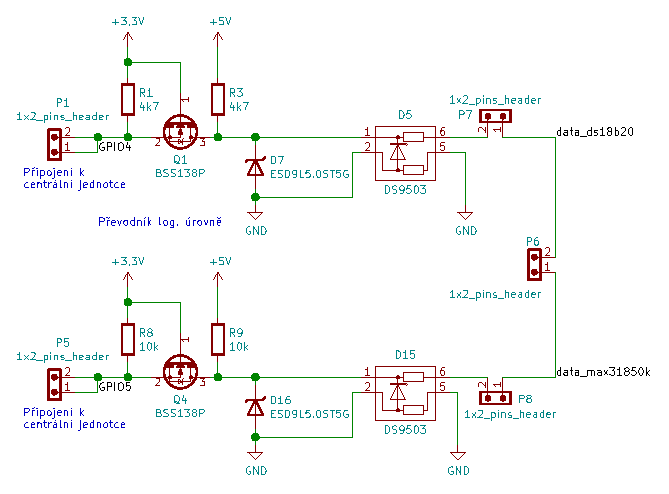
\includegraphics[width=\textwidth]{images/svg/kicad/ochrany-1-wire.eps}
    \caption[ESD ochrany pro 1-Wire sběrnici s~převodním napěťových úrovní]{ESD ochrany pro 1-Wire sběrnici s převodním napěťových úrovní. Kolíková lišta P1, P5 je připojena na Raspberry Pi.}
    \label{fig:ochrany-1-wire}
\end{figure}


\subsubsection{Napájení 1-Wire sběrnice}
\label{sec:napajeni-1-wire-sbernice}
Pro ochranu napájení 1-Wire sběrnice (5 V) jsou veškerá koncové teplotní senzory napájené přes elektronickou pojistku od Texas Instrumenst s označením TPS2600, obrázek \ref{fig:ochrana-napajeni-1-wire}. Která zajišťuje ochranu pro vstupní napětí, hlídá maximální hodnotu vstupního napětí do nastavené meze 5,25 V (maximální hranice je 60 V), minimální vstupní napětí do nastavené meze 4,75 V (minimální hranice je -60 V). Vstupní omezení napětí je pomocí rezistorů R5, R10, R11 a R12. Omezovací proud je nastaven na přibližně 73 mA (hodnotu lze změnit přes potenciometr R17), při jeho překročení dojde k odpojení výstupu pod dobu dokud nedojde k odstranění závady. Kondenzátor C2 nastavuje rychlost náběhu výstupního napětí. Pro indikaci chyb napájení je zde červená LED.

\begin{figure}[H]
    \centering
    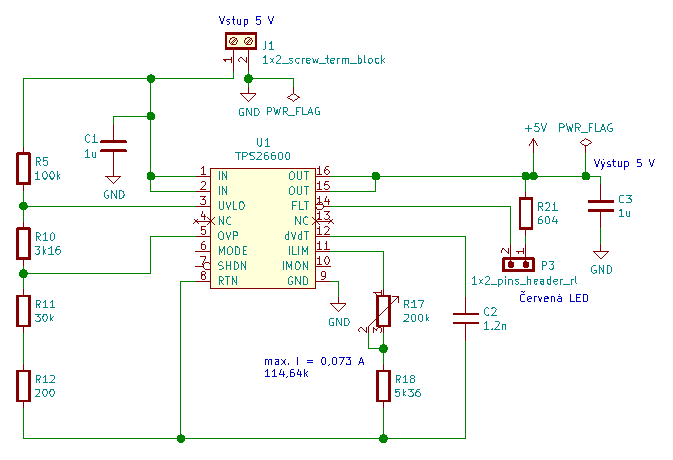
\includegraphics[width=\textwidth]{images/svg/kicad/ochrana-napajeni-1-wire.eps}
    \caption{Obvod TPS26600 pro ochranu napájení 1-Wire sběrnice.}
    \label{fig:ochrana-napajeni-1-wire}
\end{figure}

\subsubsection{Ochrana pro chodbové nástěnné termostaty}
Obdobně jako v části \ref{sec:datova-cast-1-wire-sbernice} (Datová část 1-Wire sběrnice) je stejná ochrana pro snímání logické úrovně z~chodbových nástěnných termostatů. Při sepnutí chodbového termostatu na daném patře je detekována log. 0 (požadavek na vytápění) v opačném případě je zde log. 1 (zastavení vytápění). Chodbové nástěnné termostaty jsou popsány v sekci \ref{digitalni-chodbove-termostaty}.

\subsubsection{Ochrana napájení 3,3 V}
Přímo z Raspberry Pi je využito napětí 3,3 V pro převodník napětí, popsaný v~části \ref{sec:datova-cast-1-wire-sbernice} (datová část 1-Wire sběrnice). Zde je použita vratná pojistka polymerový PTC (RXEF005) se spínacím proudem 100 mA, pro omezení proudu v~případě poruchy, dále je zde transilová dioda (SM2T3V3A) pro ochranu při přepětí (s~upínacím napětí max. 6,5 V (při 25 A, 10/1000~µs), průrazné napětí 3,6 V). Na obrázku \ref{fig:ochrana-napajeni-3_3-v} je zobrazena popsaná ochrana.

\begin{figure}[H]
    \centering
    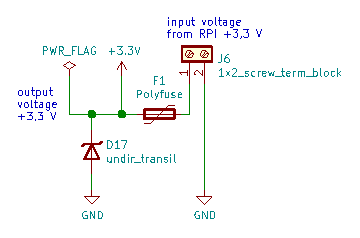
\includegraphics[width=0.6\textwidth]{images/svg/kicad/ochrana-napajeni-3_3-v.eps}
    \caption{Ochrana pro napájení 3,3 V z~Raspberry Pi.}
    \label{fig:ochrana-napajeni-3_3-v}
\end{figure}

\subsubsection{Způsob realizace 1-Wire sběrnice}
Samotná 1-Wire sběrnice je realizovaná pomocí UTP kabelu kategorie Cat5e. Na pinu číslo 4 jsou DATA, na pinu 5 je zem (GND) a na pinu 3 je napájení 5~V. Ze samotné DPS je sběrnice vyvedena pomocí konektorů RJ45, čtyři konektory pro teplotní senzory DS18B20 a čtyři pro termočlánky s MAX31850K.

\subsubsection{Realizovaná DPS ochran pro centrální jednotku Raspberry Pi}
Na obrázku \ref{fig:dps-rpi-1-wire-termostaty-ochrany-spodek} a \ref{fig:dps-rpi-1-wire-termostaty-ochrany-vrsek} je realizovaná DPS vstupů/výstupů pro centrální jednotku Raspberry Pi. Deska byla vlastnoručně navržena, vyrobena a osazena. Je aplikován ochranný lak, na vrchní propojky byl též aplikován ochranný lak a následně zakryty tavnou plastovou hmotou. Celkové schéma zapojení je v příloze \ref{app:schemata-ostatni}. Toto zařízení bylo realizováno jednou a je umístěné v rozvaděči.

\begin{figure}[H]
    \centering
    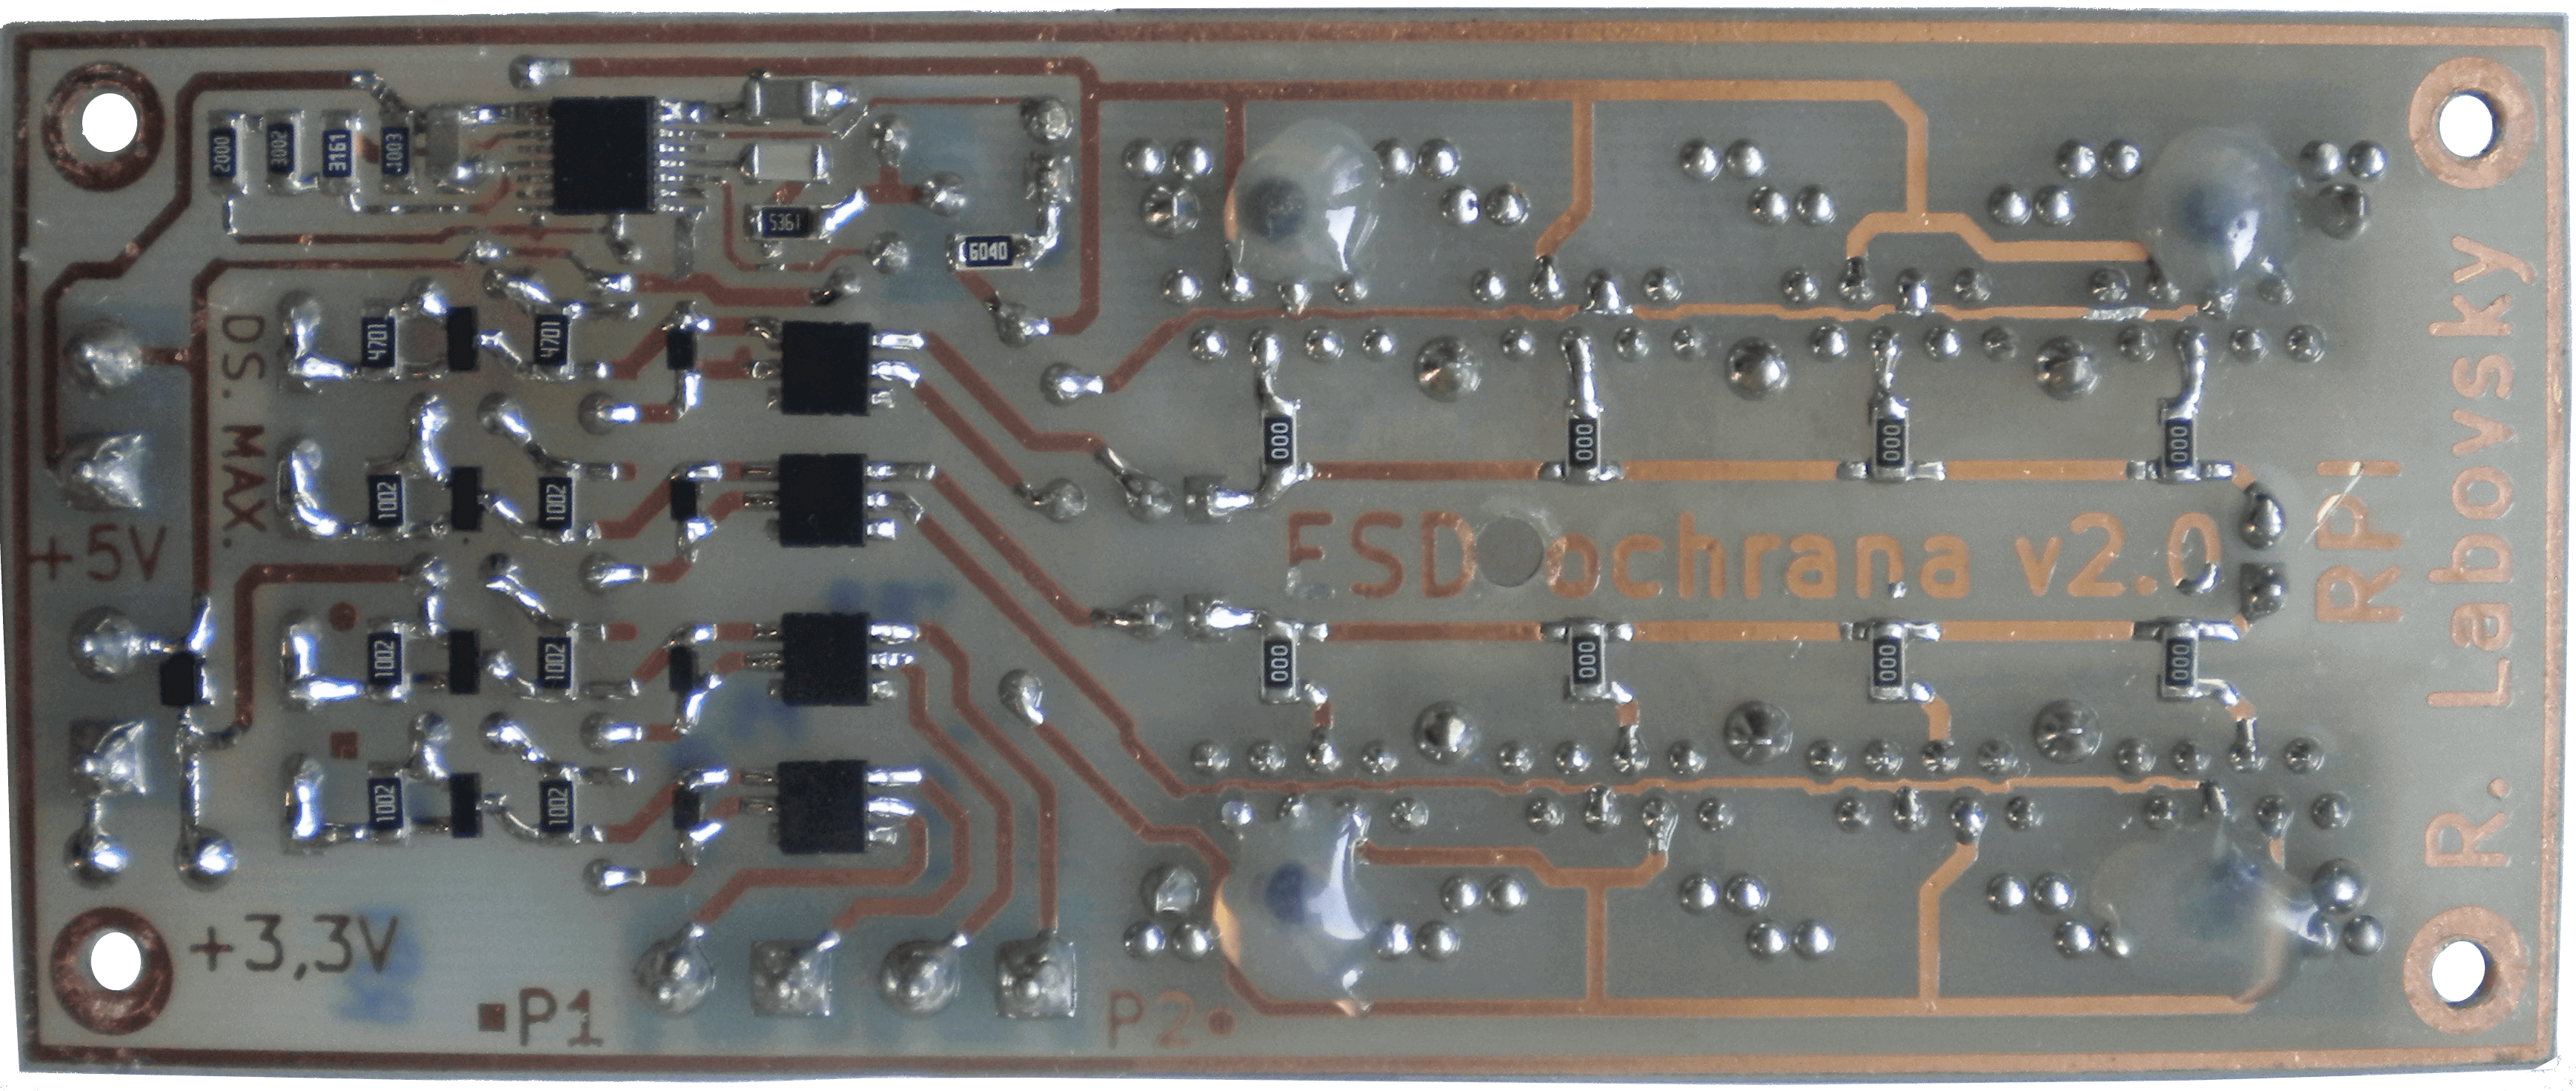
\includegraphics[width=\textwidth]{images/dps-rpi-1-wire-termostaty-ochrany-spodek.png}
    \caption{Spodní část DPS pro ochranu vstupů/výstupů pro centrální jednotku Raspberry Pi.}
    \label{fig:dps-rpi-1-wire-termostaty-ochrany-spodek}
\end{figure}

\begin{figure}[H]
    \centering
    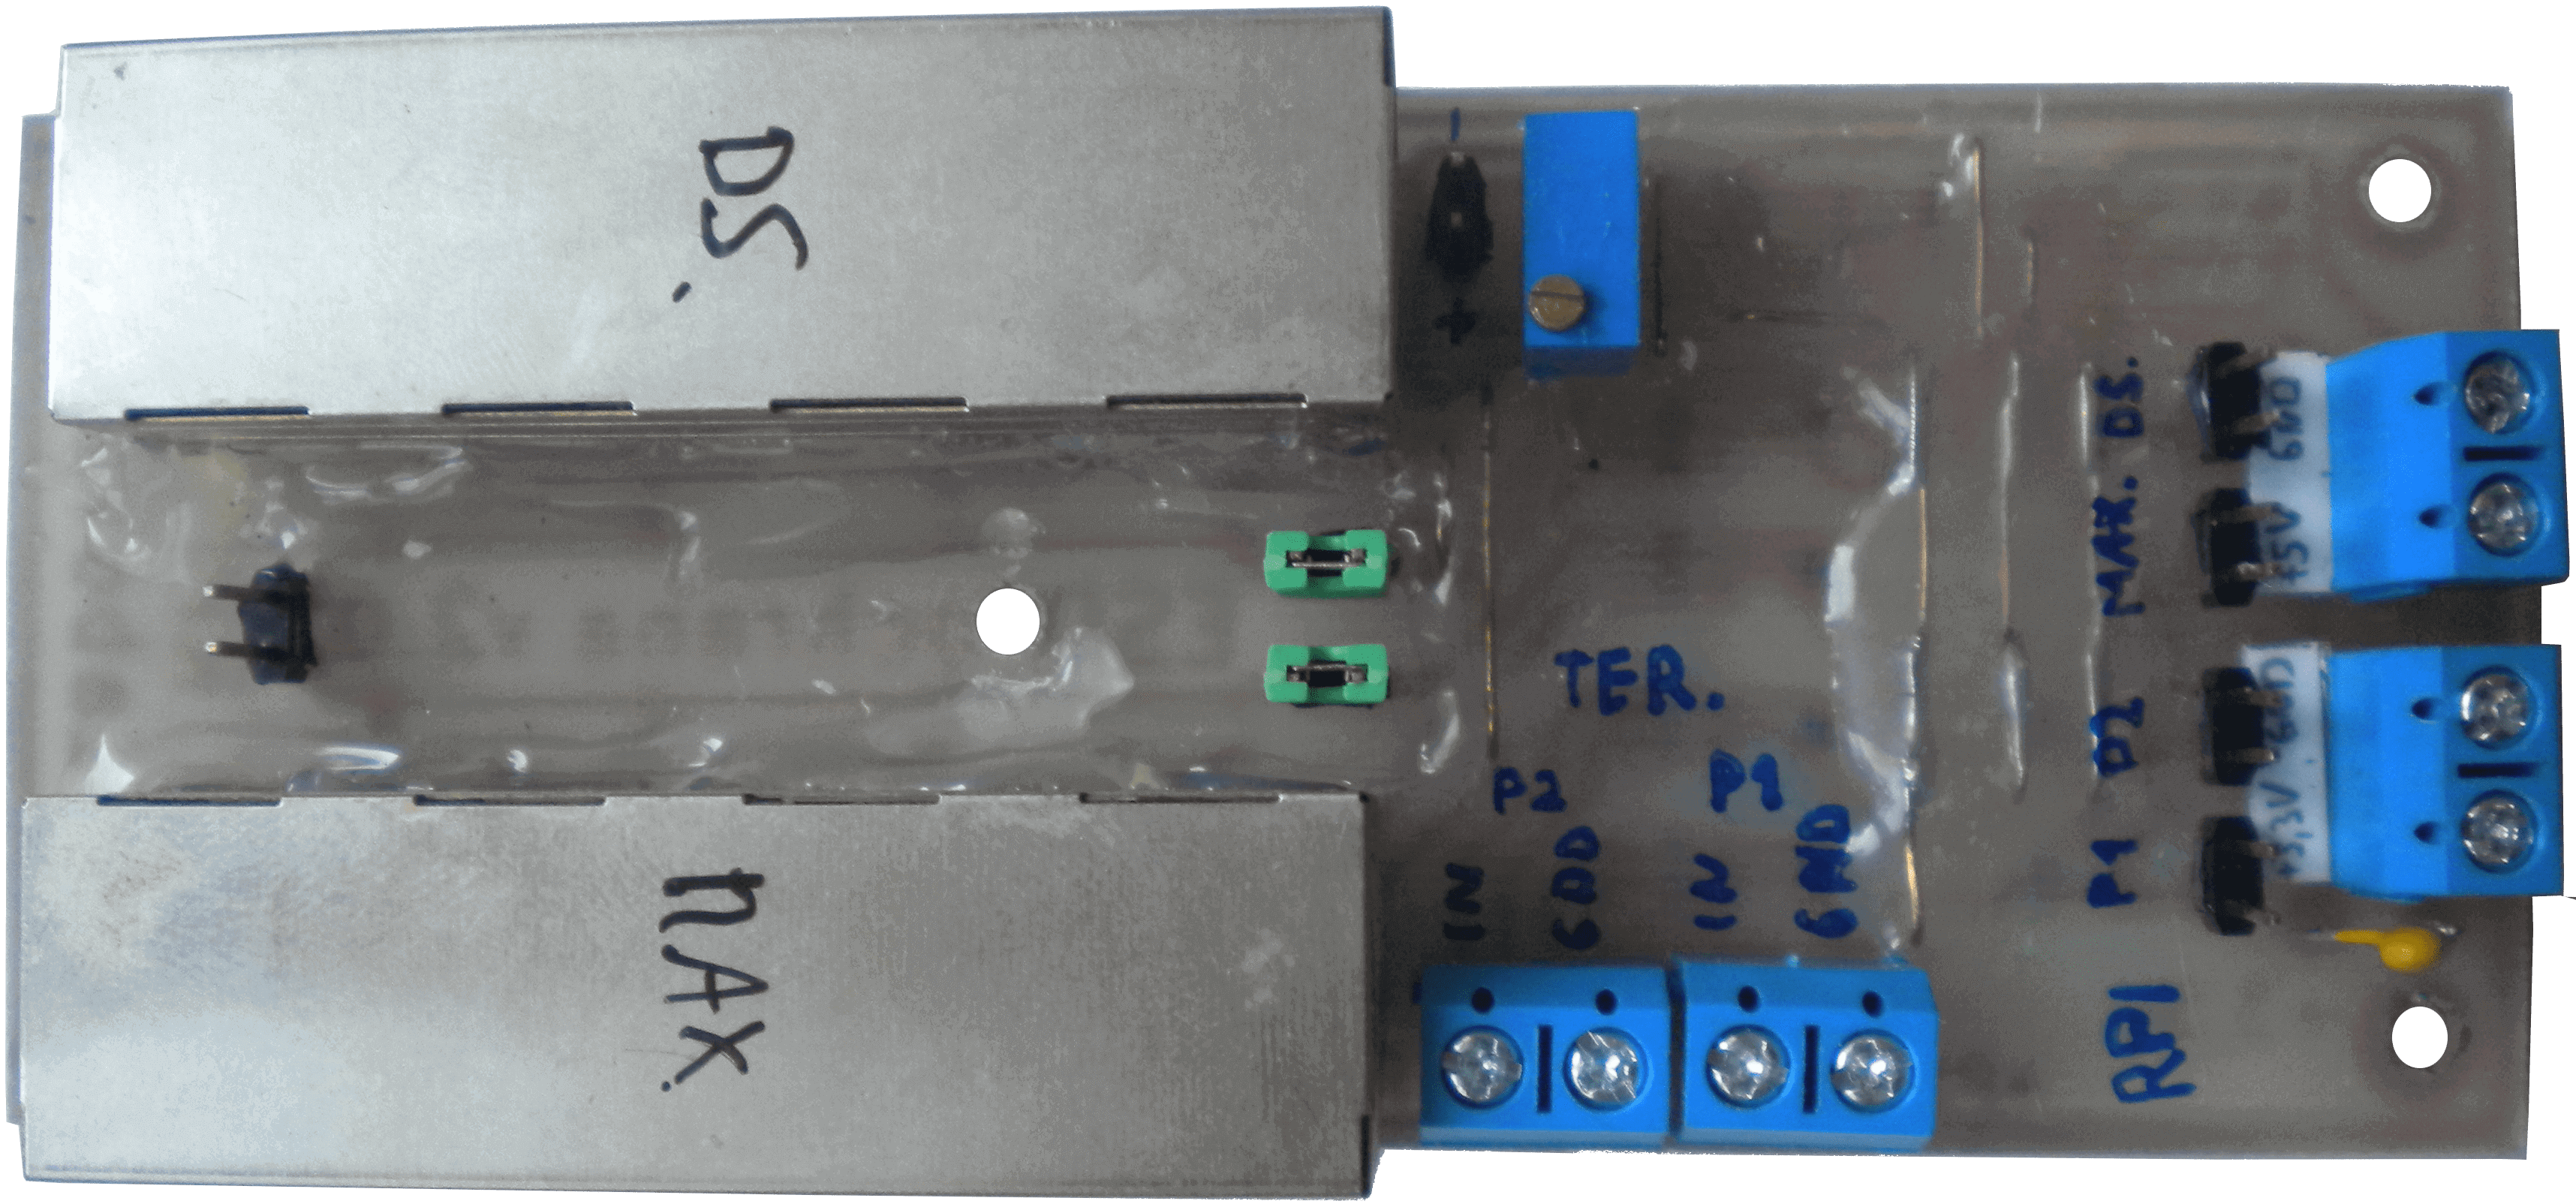
\includegraphics[width=\textwidth]{images/dps-rpi-1-wire-termostaty-ochrany-vrsek.png}
    \caption{Vrchní část DPS pro ochranu vstupů/výstupů pro Raspberry Pi.}
    \label{fig:dps-rpi-1-wire-termostaty-ochrany-vrsek}
\end{figure}